\documentclass[aspectratio=169]{beamer}
\mode<presentation>
%\usetheme{Warsaw}
%\usetheme{Goettingen}
\usetheme{Hannover}
%\useoutertheme{default}

%\useoutertheme{infolines}
\useoutertheme{sidebar}
\usecolortheme{dolphin}


\setbeamersize{sidebar width left=0pt} % to remove the sidebar
\beamertemplatenavigationsymbolsempty % To remove the navigation symbols on the bottom right.
\setbeamersize{text margin left=10mm,text margin right=10mm} % Specify margins

\usepackage{amsmath}
\usepackage{amssymb}
\usepackage{listings}
\usepackage{enumerate}
\usepackage{hyperref}
\usepackage{comment}
\hypersetup{
    colorlinks=true,
    linkcolor=blue,
    filecolor=magenta,      
    urlcolor=cyan,
}
 
\urlstyle{same}

%some bold math symbosl
\newcommand{\Cov}{\mathrm{Cov}}
\newcommand{\Var}{\mathrm{Var}}
\newcommand{\brho}{\boldsymbol{\rho}}
\newcommand{\bSigma}{\boldsymbol{\Sigma}}
\newcommand{\btheta}{\boldsymbol{\theta}}
\newcommand{\bbeta}{\boldsymbol{\beta}}
\newcommand{\bmu}{\boldsymbol{\mu}}
\newcommand{\bW}{\mathbf{W}}
\newcommand{\one}{\mathbf{1}}
\newcommand{\bH}{\mathbf{H}}
\newcommand{\by}{\mathbf{y}}
\newcommand{\bolde}{\mathbf{e}}
\newcommand{\bx}{\mathbf{x}}

\newcommand{\cpp}[1]{\texttt{#1}}

%--------------------------------------------------
\providecommand{\abs}[1]{\lvert#1\rvert}
\providecommand{\norm}[1]{\lVert#1\rVert}
\providecommand{\Blue}[1]{\textcolor{blue}{#1}}
\providecommand{\Red}[1]{\textcolor{red}{#1}}
\newcommand{\celsius}{\ensuremath{^\circ}C}
\newcommand\thfore{\mathord{\therefore}\,}
%--------------------------------------------

\title{Lecture 11. Introduction to Logic }

\author{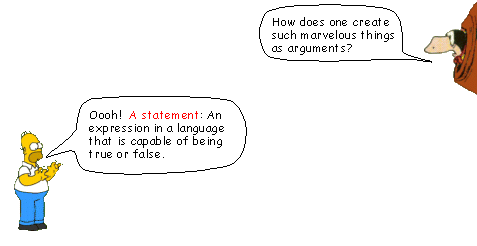
\includegraphics[width=.6\textwidth,height=.5\textheight]{./img/lecture11-fig0.png} }
   
\date{ {\tiny Figure Source: \url{http://web.csulb.edu/~cwallis/100/slides/toolkit/toolkit.html} } } 
%\date{}


%\logo{\includegraphics[height=0.5cm]{Logo_PPT.pdf}}

\begin{document}



\frame[plain]{\titlepage}


%%%%%
%\begin{comment}

\begin{frame}[plain]{ }

{\small 
The following two {\bf inquiry problems} are designed to help you begin thinking about the ideas in
the topic of logic.
 Think about them on your own
and discuss your thoughts, conclusions, and questions with your classmates.

\begin{enumerate}
%  \item Ahmed, standing with his hands behind his back, claims that he is holding a
 %   1 Dirham coin in his left hand and a 20 Dhs bill in his right hand. 
 %   You believe he is lying. What would you have to show to demonstrate that he is lying?
 %    Invent a diagram, chart, or symbols to illustrate all the possible scenarios.
  \item Maryam knows whether or not Ahmed is lying. She promises that if Ahmed is
      lying, she will give you a cookie. Maryam always keeps her promises. Suppose she does not
     give you a cookie; what can you conclude? Suppose she gives you a cookie; what can you
    conclude? % Illustrate your thinking in some organized way.
  \item Camp Halcyon and Camp Placid are two summer camps with the following daily
    policies on pool use and cleanup duties.
    \begin{itemize}
      \item Camp Halcyon's Policy: If you used the pool in the afternoon and you didn't clean up after
lunch, then you must clean up after dinner.
      \item Camp Placid's Policy: You must do at least one of the following: (a) Stay out of the pool in
      the afternoon, (b) clean up after lunch, or (c) clean up after dinner.
    \end{itemize}
    How do these policies differ? Explain your reasoning.
\end{enumerate}
}

\end{frame}

%\end{comment}
%%%%%%%%%%%%%%

\begin{frame}[plain]{What is Logic?}
 
 \begin{itemize}
  \item \Blue{Logic} is {\bf the study of reasoning}.
     It is specifically concerned with whether reasoning is correct.\pause
  \item The central concept of logic is the concept of argument form. 
    \begin{itemize}
    \item An \Blue{argument} is a
    sequence of \Blue{statements} aimed at demonstrating the truth of an assertion. 
    \item The assertion at
   the end of the sequence is called the \Blue{conclusion}, 
   and the preceding statements are called
   \Blue{premises}. 
   \item To have confidence in the conclusion that you draw from an argument, 
   you must be sure that the premises are acceptable on their own merits 
   or follow from other statements that are known to be true.
  \end{itemize}\pause
  \item Uses and Applications in Computer Science
    \begin{itemize}
       \item To prove correctness of software/hardware.
       \item Used in computer circuit design.
       \item Used in modeling programming languages.
       \item Used in the design of expert systems, robots, and artificial intelligence.
     \end{itemize}
\end{itemize}

 
\end{frame}



\begin{frame}[plain]{}

A \Blue{statement} (or \Blue{proposition}) is a sentence 
that can be {\bf either true or false}, but \Red{\bf not both}.
\pause
  A \Blue{simple statement}~\footnote{It is the basic building block of logic and
   can be called an \Blue{atomic statement}.}
    is a statement
  which cannot be broken down into simpler statements.
    
  
  \medskip
  
  {\bf Example 11.1}. Statement or not? \pause 
   \begin{itemize}
   % \item  7 is odd. \pause
     \item The moon is made of cheese. \pause
   % \item $1+1=4$ \pause
     \item 42 is a perfect square. \pause 
    \item If it is raining, then the ground is wet. \pause
  %  \item Our professor is from Mars. \pause
    \item Abu Dhabi is the capital of United Arab Emirates.
    \item $x$ is even. \pause
   % \item This sentence is false.~\footnote{Logican paradox}
    \item The sum of two squares.
       \pause
    \item Would you like some cake?\pause
%    \item What time is it? \pause
    \item Read this carefully. 
   \end{itemize}

\end{frame}


\begin{frame}[plain]{}

We can use \Blue{ statement variables} (or \Blue{propositional variables}) 
 to represent a simple statement.
For a statement variable, a lowercase letter is usually used, for example: $p,q,r,…,$
 and so on.
The truth value of a statement variable  is {\bf True} or {\bf False}.  

\medskip

{\bf Example 11.2.} 
\begin{itemize}
 \item \Blue{p}: January has 31 days.
 \item \Blue{q}: February has 33 days.
\end{itemize}

\vspace{1in}


\end{frame}

\begin{frame}[plain]{}

  {\bf Definition} A \Blue{Compound Statement}  is the combination of two or more simple statements 
   
  \medskip
  
  {\bf Example 11.3}. ``Today is Tuesday'' and ``Tomorrow is holiday''.
  \medskip
  \pause
  
  A compound statement consists of several simple statements joined together by words such 
 as ``{\bf and}'', ``{\bf or}'', ``{\bf if ... then}'', etc. 
 These {\bf connecting words} are represented by the five 
 \Blue{logical connectives} 
 \begin{center}
   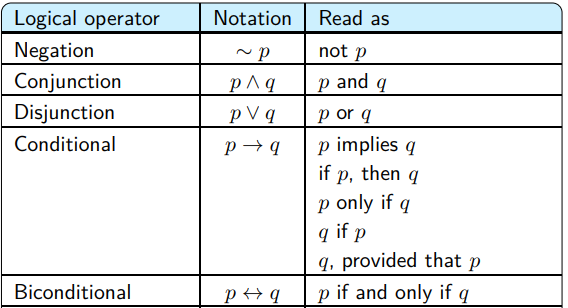
\includegraphics[height=4.3cm]{./img/lecture11-fig1.png}
 \end{center}

\end{frame}

\begin{frame}[plain]{Negation}

\begin{itemize}
 \item  Consider the {\bf statement}
    
    \begin{itemize}
       \item $p$:  Discrete Math is a required course for sophomores.
    \end{itemize}
 
 \item The \Blue{negation} of  $p$ is denoted by $\neg p$
 and is read ``\Blue{\emph{ not p}}''. 
   \begin{itemize}
       \item $\neg p$:  ``Discrete Math is not a required course for sophomores" 
        \ \  or \ \ ``It is not the case that Discrete Math is a required course for 
 sophomores.''
    \end{itemize}
 \pause 
    \item \Blue{Truth Table}
        \begin{center}
          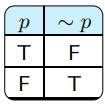
\includegraphics[height=1.7cm]{./img/lecture11-fig2.png}
        \end{center}

\end{itemize}

{\bf Example 11.4.} Let $p:$ represent ``$x$ is a real number such that $x<4$." 
    Then $\neg p$: \pause ``$x$ is a real number such that $x\geq4$." 

\vspace{.5in}

\end{frame}


\begin{frame}[plain]{Conjunction }

\Blue{Conjunction}: The conjunction of the statements $p$, $q$ is denoted 
        by \Blue{$p\wedge q$}, which is read ``{\bf p and q}.'' 
 \medskip
 
 Consider the statements:
 \begin{itemize}
    \item $p$: Sam is poor.
    \item $q$: Sam is happy. 
 \end{itemize}
 
 There are many ways to express the proposition $p\wedge q$ in English:\pause 
 \begin{itemize}
  \item $p\wedge q$ = Sam is poor and he is happy. \pause
  \item $p\wedge q$ = Sam is poor, but he is happy.
  \item $p\wedge q$ = Despite the fact that he is poor, Sam is happy.
  \item $p\wedge q$ = Although Sam is poor, he is happy.
 \end{itemize}
 
 \medskip
 
 What are the truth values of $p\wedge q$?
 \end{frame}
 

\begin{frame}[plain]{}

 Truth Table of $p\wedge q$:
 
              \begin{center}
                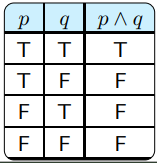
\includegraphics[height=2.5cm]{./img/lecture11-fig3.png}
              \end{center}               

{\bf Example 11.5.} Write $0\leq x\leq 1$ using conjunction: \pause 
        $(x\geq 0) \wedge (x\leq 1)$.
        
     \vspace{.7in}
     

\end{frame}


\begin{frame}[plain]{Disjunction (Inclusive or)}

\begin{itemize}[<+->]
 \item \Blue{Disjunction} ({\bf Inclusive or}): The expression \Blue{$\mathbf{p\vee q}$} denotes the {\bf disjunction}
   of the statements $p, q$ and is read {\bf p or q}. In particular, this is {\bf inclusive}.
   \begin{itemize}
      \item $p\vee q$ ({\bf Inclusive or}): ``Students who have taken calculus or computer science can
            take this class.''
      \item Truth Tables of \Blue{Inclusive or} ($\mathbf{p\vee q}$)       
          \smallskip
          
              \begin{center}
                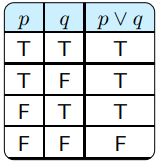
\includegraphics[height=2.7cm]{./img/lecture11-fig4.png}
              \end{center}  
        \end{itemize}
    \end{itemize}
\end{frame}

\begin{frame}[plain]{Disjunction (Exclusive or = XOR)}

\begin{itemize}[<+->]
 \item \Blue{Disjunction} (Exclusive or): The expression \Blue{$p\oplus q$} denotes the {\bf disjunction}
   of the statements $p, q$ and is read {\bf p or q}. In particular, this is {\bf exclusive}.
 \item When a menu at a restaurant states, ``Soup or salad comes with an entrée,''
      the restaurant almost always means that customers can have  
      \mbox{\_\_\_\_\_\_\_\_\_}.%either soup or salad, but not both. 
      \  Hence, this is an exclusive or rather than an inclusive or.
 \item Truth Tables of  \Blue{Exclusive or} 
   ($\mathbf{p\oplus q} \ \Blue{\equiv}\ (p\vee q)\wedge \neg(p\wedge q)$)
              \begin{center}
                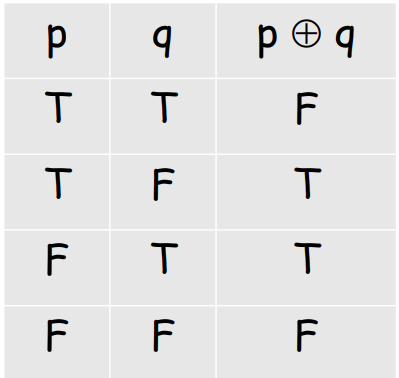
\includegraphics[height=3cm]{./img/lecture11-fig5.png}
              \end{center}  
 \item {\bf Example 11.6.} $p\oplus q$: ``Students who have taken calculus or computer science, but not both,
            can enroll in this class.''
\end{itemize}
\end{frame}


\begin{frame}[plain]{Conditional Statement}

\begin{itemize}[<+->]
 \item \Blue{Conditional Statement}: The conditional statement \Blue{$p\rightarrow q$} 
   is the proposition {\bf if  p, then q}. 
 \item $p$ is called a \Blue{premise} (or \Blue{hypothesis}) and $q$ is called a 
    \Blue{conclusion}.
      \item {\bf Example 11.7.} $p\rightarrow q$ = ``If you get 100\% on the final, then
          you will get an A''
    
      \item Truth Table 
      
              \begin{center}
                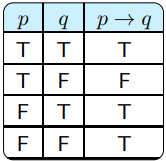
\includegraphics[height=2.7cm]{./img/lecture11-fig6.png}
              \end{center}  
       \item If you manage to get a 100\% on the final, then you would expect to receive an A. 
         If you do not get 100\% you may or may not receive an A depending on 
       other factors. However, if you do get 100\%, 
         but the professor does not give you an A, you will feel cheated. 
  
    \end{itemize}
\end{frame}

\begin{frame}[plain]{}

\begin{itemize}
   \item Because conditional statements play such an essential role in mathematical reasoning, 
     a variety of terminology is used to express $p\rightarrow q$. 
     \begin{enumerate}
      \item ``\Blue{if p, then q}''; ``\Blue{p implies q}'';
           ``\Blue{q if p}''; ``\Blue{q whenever p}''; ``\Blue{q when p}''
      \item ``\Blue{p is sufficient for q}''; ``\Blue{a sufficient condition for q is p}''
      \item ``\Blue{q is necessary for p}'';
             ``\Blue{a necessary condition for p is q}'';
         ``\Blue{q follows from p}''
      \item ``\Blue{p only if q}'' = \Red{p cannot be true when q is not true}; that is, the statement is false
          if p is true but q is false.~\footnote{In other words,
            p only if q means that the truth of q is necessary, or required, in order for p to be true.
              That is, p only if q rules out just one possibility: that p is true and q is false. 
              But that is exactly what $p\rightarrow q$ rules out.
              So it’s obviously correct to read $p\rightarrow q$ as p only if q.}
          When p is false, q may be either true or false, 
           because the statement says nothing about the truth value of q.
  %    \item ``\Blue{q unless        $\neg p$}'' = if $\neg p$ is false, then q must be true
  %           = ``q unless $\neg p$'' is false when p is true but q is false, but it is true otherwise.
  %           (Meaning of {\bf unless}~\footnote{except if (used to introduce the case in which 
  %      a statement being made is not true or valid).
  %   ''Unless you have a photographic memory, repetition is vital``})
     \end{enumerate} 
    \end{itemize}
\end{frame}

\begin{frame}[plain]{}

{\bf Example 11.8.}  To get really clear on the difference between {\bf if} and {\bf only if}, consider the following sentences:

\begin{itemize}
  \item[(a)] $a$ and $b$ are the same size if $a=b$.
      \[ a = b \rightarrow \mathrm{SameSize}(a, b) \]
  \item[(b)]  $a$ and $b$ are the same size only if $a=b$.
      \[ \mathrm{SameSize}(a, b) \rightarrow a = b \]
\end{itemize}  
\pause

(a) is a logical truth: if $a$ and $b$ are one and the same object, then there is no difference between $a$ and $b$ 
    in size, shape, location, or anything else.\pause
\smallskip

(b) But (b) makes a substantive claim that could well be false: it is possible for $a$ and $b$ to be the same size 
   but be two different objects. $a$ and $b$ might be a pair of large cubes, 
    or $a$ might be a large cube and $b$ a large tetrahedron.

\end{frame}


\begin{frame}[plain]{}

\begin{itemize}
    \item {\bf Example 11.9.} Express the statement $p\rightarrow q$ with
    \begin{itemize}
       \item $p$:  Maria learns discrete math.
       \item $q$:  Maria will get a good job.
    \end{itemize}
    \pause 
    
      \begin{enumerate}[<+->]
       \item If Maria learns discrete math, then she will find a good job. 
       \item Maria will find a good job when she learns discrete math.
       \item For Maria to get a good job, it is sufficient for her to learn discrete mathematics.
       \item Maria will find a good job unless~\footnote{unless = if not} 
             she does not learn discrete math.
      \end{enumerate}
      
    
  % \item {\bf Remark 1} Conditional statements are more general than the meaning attached to
  %    statements in the English language.
  % \item {\bf Remark 2} The {\bf if-then} construction used in many programming language
  %     is different from that used in logic.

    \end{itemize}
    
    \vspace{0.8in}
    
\end{frame}

\begin{frame}[plain]{Biconditional Statement }

\begin{itemize}[<+->]
 \item \Blue{Biconditional Statement}, \Blue{$p\leftrightarrow q$}, 
   is the proposition {\bf p if and only if q}.
  \item Truth Table 
    
              \begin{center}
                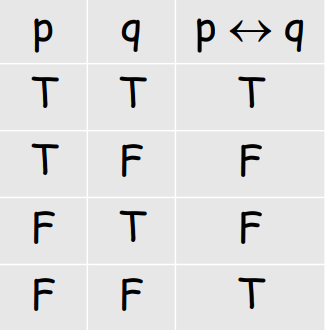
\includegraphics[height=3cm]{./img/lecture11-fig7.png}
              \end{center}  
  \item {\bf Example 11.10.} $p\leftrightarrow q$ = ``You can take the flight if and only if you buy a ticket.''
  \item Other expression: 
    ``\Blue{p is necessary and sufficient for q}''; ``\Blue{if p then q, and conversely}'';
      ``\Blue{p iff q}.'' 
    \end{itemize}
\end{frame}

\begin{frame}[plain]{ Summery of logical connectives}

\begin{center}
 
  
                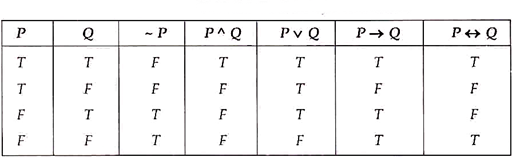
\includegraphics[height=3cm]{./img/lecture11-fig8.png}
              \end{center} 

\begin{itemize}
 \item {\small We can use these connectives
to build up complicated compound statements involving any number of propositional
variables.} 
 \item {\small Then, we can use truth tables to determine the truth values of these compound statements.}
  \item {\bf Practice 11.11} Construct the truth table of the compound statement
       \[ \Blue{(p\wedge \neg q) \rightarrow (p\vee q)}. \]
    \end{itemize}
\end{frame}

\end{document}




\begin{frame}[plain]{ }

\begin{center}
  
                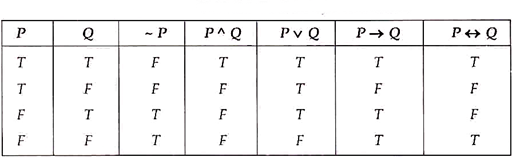
\includegraphics[height=3cm]{./img/lecture11-fig8.png}
         \end{center} 

% {\bf Problem.} Construct the truth table of the compound statement
%       \[ \Blue{(p\vee \neg q) \rightarrow (p\wedge q)}. \]  --> Changed to Quiz 1
 
\end{frame}

 
